\exercise{7|1}{Ursachen für wachsende Bedeutung des Personalmanagements}
Was sind die zentralen Ursachen für die wachsende Bedeutung des Personalmanagements?

\solution{
\begin{enumerate}
    \item \textbf{Zunehmende Größe und Komplexität vieler Unternehmen}
    \begin{itemize}
        \item Die zunehmende Größe und Komplexität vieler Unternehmen bewirkt, dass personalpolitische Maßnahmen nicht nur allein der Personaladministration dienen, sondern auch eine wichtige Koordinationsfunktion übernehmen.
        \item Verbindliche Kriterien der Personalauswahl, gruppenorientierte Formen des Personaleinsatzes und die Personalführung mit Hilfe von Zielvorgaben tragen dazu bei, die Handlungen der einzelnen Mitarbeitenden aufeinander abzustimmen und eine konsistente Unternehmenspolitik zu gewährleisten.
    \end{itemize}
    \item \textbf{Rapider Anstieg der absoluten und relativen Personalaufwendungen}
    \begin{itemize}
        \item In Deutschland und vielen anderen Ländern ist in den letzten Jahren ein rapider Anstieg der absoluten und relativen Personalaufwendungen zu beobachten.
        \item Besonders im Dienstleistungssektor nehmen die Personalaufwendungen einen bedeutenden Teil der Gesamtaufwendungen ein.
        \item Dies erfordert eine intensive Auseinandersetzung mit personalpolitischen Fragestellungen.
    \end{itemize}
    \item \textbf{Verschärfung und Globalisierung des Wettbewerbs}
    \begin{itemize}
        \item Aufgrund des steigenden Wettbewerbs werden personalpolitische Instrumente immer stärker einer ökonomischen Kosten-Nutzen-Analyse unterzogen.
        \item Es wird dabei verstärkt Wert auf Strategien zur Kostensenkung gelegt.
        \item Insbesondere Branchen, die im internationalen Wettbewerb stehen, sind davon betroffen.
    \end{itemize}
    \item \textbf{Individualisierung}
    \begin{itemize}
        \item Mitarbeitende legen zunehmend Wert auf individuelle Arbeitsbedingungen und maßgeschneiderte Entwicklungsmöglichkeiten.
    \end{itemize}
    \item \textbf{Wertewandel}
    \begin{itemize}
        \item Werte wie Nachhaltigkeit und soziale Verantwortung gewinnen an Bedeutung und beeinflussen die Ausrichtung des Personalmanagements.
    \end{itemize}
    \item \textbf{Strukturelle Veränderungen des Arbeitsmarktes}
    \begin{itemize}
        \item Es herrscht ein Mangel an qualifizierten Fachkräften (z. B. in Handwerksberufen oder der IT) bei gleichzeitig hoher Arbeitslosigkeit in anderen Bereichen.
        \item Aufgrund demographischer Entwicklungen wird sich dieses strukturelle Ungleichgewicht weiter verschärfen.
        \item Personalmanagement erfordert daher einen zielgruppenspezifischen Einsatz der Instrumente, um attraktive Beschäftigungsangebote zu schaffen.
    \end{itemize}
    \item \textbf{Digitalisierung und Entwicklung neuer Technologien}
    \begin{itemize}
        \item Die Digitalisierung fördert die Virtualisierung der Arbeit und die Mobilität der Mitarbeitenden.
        \item Dies führt zu erheblichen Änderungen von Tätigkeitsprofilen und erhöht die Bedeutung des Personalmanagements für die Anpassung an diese neuen Gegebenheiten.
    \end{itemize}
\end{enumerate}
}


\exercise{7|2}{Besondere aktuelle Herausforderungen}
Was sind die besonderen Herausforderungen, mit denen das Personalmanagement aktuell (und dabei insbesondere seit Beginn der COVID-19-Pandemie) konfrontiert ist?

\exercise{7|3}{Personalbeschaffung}
Sie sind Personalchefin der Chemix AG. Dieses Unternehmen handelt mit chemischen Rohstoffen.  
In der Abteilung „Lösungsmittel“ ist die Stelle des Verkaufsleiters zu vergeben.  
Was spricht für die Besetzung dieser Stelle mit einer betriebseigenen Arbeitskraft, was dagegen?

\solution{
\textbf{Gründe, die dafür sprechen, sind:}
\begin{itemize}
    \item Betriebseigene Mitarbeitende sind bereits in den Betrieb integriert und mit den Geschäftspflichten und der Unternehmenskultur vertraut.
    \item Die Unternehmensleitung kennt sowohl die Leistungen und Fähigkeiten als auch die Schwächen der internen Bewerberinnen und Bewerber.
    \item Die interne Lösung bietet einen Anreiz für Mitarbeitende, da sie eine Beförderung anstreben und sich stärker motiviert für ihre Arbeit einsetzen.
    \item Es ist keine aufwändige Einarbeitung notwendig.
    \item Die interne Lösung erlaubt unter Umständen eine schnellere Realisierung.
\end{itemize}


\textbf{Gründe, die dagegen sprechen, sind:}
\begin{itemize}
    \item Neue Mitarbeitende bringen neue Ideen und Erfahrungen mit.
    \item Eventuelle interne Intrigen können entschärft werden.
    \item Ein Vergleich mit den Qualifikationen und Forderungen externer Arbeitskräfte ist möglich.
    \item Es lassen sich wichtige Kenntnisse über die Stellung des Unternehmens im Arbeitsmarkt gewinnen.
    \item Insgesamt müssen nun zwei Stellen neu besetzt werden.
\end{itemize}
} 

\exercise{7|4}{Unterdeckung bzw. Überdeckung des Fähigkeitsprofils}
Was unternehmen Sie als Vorgesetzte, wenn das Fähigkeitsprofil Ihrer Mitarbeitenden gegenüber dem Anforderungsprofil eine Unterdeckung bzw. Überdeckung aufweist?
\solution{

\textbf{Maßnahmen, die bei einer Unterdeckung zu ergreifen sind:}
\begin{itemize}
    \item Geeignete Personalentwicklungsmaßnahmen
    \item Einsatz an einer anderen, den Fähigkeiten entsprechenden Stelle
    \item Personalfreistellung
\end{itemize}

\textbf{Maßnahmen, die bei einer Überdeckung zu ergreifen sind:}
\begin{itemize}
    \item Einsatz an einer anderen, höher qualifizierten Stelle
    \item Ausweitung des Tätigkeitsbereichs
\end{itemize}
}

\exercise{7|5}{Jobsharing}
Seit einiger Zeit verstärkt sich das Bedürfnis nach neuen Arbeitsformen.  
Zu erwähnen ist in diesem Zusammenhang zum Beispiel das Jobsharing*.  

\textit{* Jobsharing bedeutet, dass mehrere Arbeitskräfte sich eine oder mehrere Stellen teilen. Das Team ist als Ganzes verantwortlich für die zu erledigenden Arbeiten. Es ist in der Aufteilung der Arbeitszeit im vorgegebenen Rahmen autonom.}  


\textbf{Beispiele:}  
\begin{itemize}
    \item Doppelbesetzungen von Lehrerstellen
    \item Doppelbesetzungen von Kindergärtnerstellen
    \item Zwei Sekretäre teilen sich eine Stelle
    \item Mehrere Krankenpfleger teilen sich eine Stelle
    \item Teilung einer Schicht in der Produktion
    \item Zwei Professoren teilen eine Stelle
\end{itemize}

\textbf{Aufgaben:}  
\begin{enumerate}[label=(\alph*)]
    \item Beschreiben Sie Vor- und Nachteile dieser Arbeitsform.
    \item Welches sind die Voraussetzungen, um das Jobsharing anwenden zu können?
\end{enumerate}
\solution{
  \textbf{a)}
\textbf{VORTEILE}
\begin{itemize}
    \item \textbf{Für die Arbeitnehmer:}
    \begin{itemize}
        \item Kleinere und flexiblere Arbeitszeitbelastung
        \item Mitarbeitende mit Teilzeitbeschäftigung können gefördert werden
    \end{itemize}
    \item \textbf{Für den Arbeitgeber:}
    \begin{itemize}
        \item Senkung der Fehl- und Fluktuationsrate (zum Teil wegen Stellvertretungspflicht)
        \item Höhere Produktivität aufgrund steigender Motivation
        \item Höhere Effizienz der Stelleninhaber, weil sie Aufgaben und Funktionen nach ihren Fähigkeiten übernehmen können
        \item Permanente Besetzung des Arbeitsplatzes
        \item Erfahrung und Wissen mehrerer Personen größer als die einer einzelnen Person
        \item Einsparungspotenzial bei der Personalaufgabe
        \item Zusammenarbeit kann Arbeitsklima und damit Leistung fördern
    \end{itemize}
\end{itemize}

\textbf{NACHTEILE}
\begin{itemize}
    \item Oft unklare Verantwortung nach außen
    \item Kommunikationsschwierigkeiten möglich
    \item Höhere Kosten bei Administration, Sozialleistungen und Weiterbildung
    \item Wirkung der Konflikte im Team vordergründig stärker als in einer hierarchischen Struktur
    \item Unterschiedliche Arbeitsproduktivität und -qualität der Job Sharer
    \item Probleme bei unerwartetem Stellenwechsel
\end{itemize}

\textbf{b)}

\begin{itemize}
    \item Klare und verbindliche Vereinbarungen zwischen den Job Sharern
    \item Transparenz bei der Aufgabenverteilung und Verantwortungsbereichen
    \item Bereitschaft der Mitarbeitenden zur Teamarbeit
    \item Effektive Kommunikationsstrukturen
    \item Unterstützung durch die Personalabteilung für administrative Fragen
    \item Anpassung der Unternehmenskultur an flexible Arbeitsmodelle
\end{itemize}
}
\exercise{7|6}{Leistungsabhängige Vergütung (Teamanreize)}
Sie haben sich entschieden, Ihre Vergütung leistungsabhängig in Form von Teamanreizen zu gestalten.  
Erläutern Sie mögliche Schwierigkeiten, die auf Sie zukommen könnten, und beschreiben Sie, wie Sie auf diese reagieren würden.
\solution{
\textbf{Mögliche Schwierigkeiten bei der Einführung von Teamanreizen können sein:}
\begin{itemize}
    \item Das zu erreichende Gruppenziel ist nicht für alle Mitglieder transparent.
    \item Die bestehende Unternehmenskultur verhindert eine Zusammenarbeit und gegenseitige Unterstützung.
    \item Das Team ist in seiner Zusammensetzung hinsichtlich Interessen und Leistungsvermögen zu heterogen.
    \item Es fehlt an dem Gefühl, in der Gruppe aufeinander angewiesen zu sein, um als Team erfolgreich zu sein.
    \item Die Zusammenarbeit ist zu kurz, um eine Vertrauensbasis im Team entstehen zu lassen.
    \item Im Team entwickeln sich manche Teilnehmer zu „Trittbrettfahrern“.
\end{itemize}

\textbf{Mögliche Maßnahmen zur Lösung dieser Schwierigkeiten:}
\begin{itemize}
    \item Klare und transparente Kommunikation der Gruppenziele und der Vergütungsregeln.
    \item Förderung einer kooperativen Unternehmenskultur durch Workshops und Teambuilding-Maßnahmen.
    \item Ausgewogene Zusammensetzung der Teams, um eine Balance aus Fähigkeiten und Interessen zu schaffen.
    \item Langfristige Zusammenarbeit im Team fördern, um Vertrauen aufzubauen.
    \item Einführung von Mechanismen, um Trittbrettfahrer zu identifizieren und zu vermeiden, z. B. durch regelmäßige Leistungsbewertungen.
    \item Kontinuierliche Evaluation und Anpassung der Teamanreize auf Basis von Feedback der Mitarbeitenden.
\end{itemize}
}
\exercise{7|7}{Personalfreistellung}
Viele Unternehmen stehen aus verschiedenen Gründen vor der schwierigen Aufgabe, Personal entlassen zu müssen.

\begin{enumerate}[label=(\alph*)]
    \item Versuchen Sie zu zeigen, welche Maßnahmen bei welchen Ursachen der Personalfreistellung sinnvoll sind.
    \item Welches sind die Folgen einer unfreiwilligen Kündigung sowohl für den Arbeitnehmer (Mitarbeitende) als auch für den Arbeitgeber (Unternehmen)?
\end{enumerate}

\begin{figure}[H]
    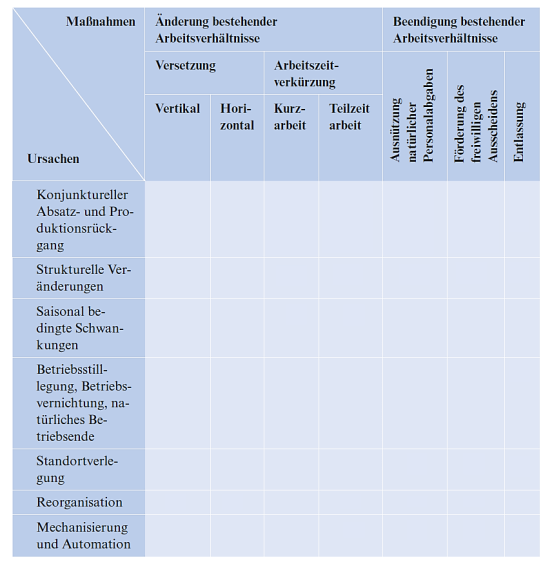
\includegraphics[width=0.55\textwidth]{figures/7_7.png} % Replace with your graphic path
\end{figure}
\solution{
\textbf{a) Maßnahmen bei Personalfreistellung:}
\begin{figure}[H]
    \centering
    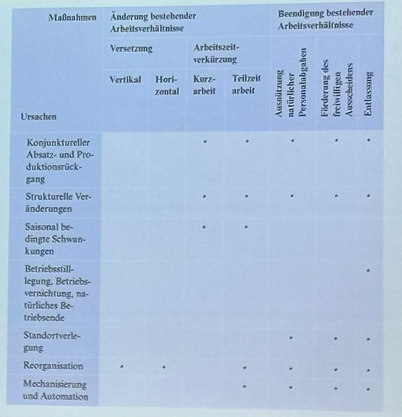
\includegraphics[width=\textwidth]{figures/7_7_2.png}
    \caption{Maßnahmen bei Personalfreistellung}
\end{figure}

\textbf{b) Folgen einer unfreiwilligen Kündigung:}

\textbf{Für die Arbeitnehmer:}
\begin{itemize}
    \item Senkung des Lebensstandards
    \item Verlust der beruflichen Anerkennung
    \item Verlust sozialer Kontakte (Familie, Freundeskreis)
    \item Mögliche Langzeitarbeitslosigkeit
    \item Gesundheitliche Probleme (psychisch oder physisch)
\end{itemize}

\textbf{Für die Arbeitgeber:}
\begin{itemize}
    \item Imageverlust für das Unternehmen
    \item Verschlechterung des Betriebsklimas
    \item Kosten für den Sozialplan
    \item Die genannten negativen Folgen machen die Notwendigkeit eines Outplacement deutlich.
\end{itemize}
}
